% interactcadsample.tex
% v1.04 - May 2023

\documentclass[]{interact}

\usepackage{epstopdf}% To incorporate .eps illustrations using PDFLaTeX, etc.
\usepackage{subfigure}% Support for small, `sub' figures and tables
%\usepackage[nolists,tablesfirst]{endfloat}% To `separate' figures and tables from text if required

\usepackage{natbib}% Citation support using natbib.sty
\bibpunct[, ]{(}{)}{;}{a}{}{,}% Citation support using natbib.sty
\renewcommand\bibfont{\fontsize{10}{12}\selectfont}% Bibliography support using natbib.sty

\theoremstyle{plain}% Theorem-like structures provided by amsthm.sty
\newtheorem{theorem}{Theorem}[section]
\newtheorem{lemma}[theorem]{Lemma}
\newtheorem{corollary}[theorem]{Corollary}
\newtheorem{proposition}[theorem]{Proposition}

\theoremstyle{definition}
\newtheorem{definition}[theorem]{Definition}
\newtheorem{example}[theorem]{Example}

\theoremstyle{remark}
\newtheorem{remark}{Remark}
\newtheorem{notation}{Notation}


% tightlist command for lists without linebreak
\providecommand{\tightlist}{%
  \setlength{\itemsep}{0pt}\setlength{\parskip}{0pt}}



\usepackage{lscape}
\usepackage{hyperref}
\usepackage[utf8]{inputenc}
\def\tightlist{}
\usepackage{setspace}
\doublespacing

\usepackage{booktabs}
\usepackage{longtable}
\usepackage{array}
\usepackage{multirow}
\usepackage{wrapfig}
\usepackage{float}
\usepackage{colortbl}
\usepackage{pdflscape}
\usepackage{tabu}
\usepackage{threeparttable}
\usepackage{threeparttablex}
\usepackage[normalem]{ulem}
\usepackage{makecell}
\usepackage{xcolor}

\begin{document}


\articletype{}

\title{Appendix to ``Automated Assessment of Residual Plots with
Computer Vision Models''}


\author{\name{Weihao Li$^{a, b}$, Dianne Cook$^{a}$, Emi Tanaka$^{a, b,
c}$, Susan VanderPlas$^{d}$, Klaus Ackermann$^{a}$}
\affil{$^{a}$Department of Econometrics and Business Statistics, Monash
University, Clayton, VIC, Australia; $^{b}$Biological Data Science
Institute, Australian National University, Acton, ACT,
Australia; $^{c}$Research School of Finance, Actuarial Studies and
Statistics, Australian National University, Acton, ACT,
Australia; $^{d}$Department of Statistics, University of Nebraska,
Lincoln, Nebraska, USA}
}


\maketitle

\begin{abstract}
Plotting the residuals is a recommended procedure to diagnose deviations
from linear model assumptions, such as non-linearity,
heteroscedasticity, and non-normality. The presence of structure in
residual plots can be tested using the lineup protocol to do visual
inference. There are a variety of conventional residual tests, but the
lineup protocol, used as a statistical test, performs better for
diagnostic purposes because it is less sensitive and applies more
broadly to different types of departures. However, the lineup protocol
relies on human judgment which limits its scalability. This work
presents a solution by providing a computer vision model to automate the
assessment of residual plots. It is trained to predict a distance
measure that quantifies the disparity between the residual distribution
of a fitted classical normal linear regression model and the reference
distribution, based on Kullback-Leibler divergence. From extensive
simulation studies, the computer vision model exhibits lower sensitivity
than conventional tests but higher sensitivity than human visual tests.
It is slightly less effective on non-linearity patterns. Several
examples from classical papers and contemporary data illustrate the new
procedures, highlighting its usefulness in automating the diagnostic
process and supplementing existing methods.
\end{abstract}

\begin{keywords}
statistical graphics; data visualization; visual inference; computer
vision; machine learning; hypothesis testing; reression analysis;
cognitive perception; simulation; practical significance
\end{keywords}

\section{Data Generation}\label{sec-model-data-generation}

\subsection{Simulation Scheme}\label{simulation-scheme}

While observational data is frequently employed in training models for
real-world applications, the data generating process of observational
data often remains unknown, making computation for our target variable
\(D\) unattainable. Consequently, the computer vision models developed
in this study were trained using synthetic data, including 80,000
training images and 8,000 test images. This approach provided us with
precise label annotations. Additionally, it ensured a large and diverse
training dataset, as we had control over the data generating process,
and the simulation of the training data was relatively cost-effective.

We have incorporated three types of residual departures of linear
regression model in the training data, including non-linearity,
heteroskedasticity and non-normality. All three departures can be
summarized by the data generating process formulated as

\begin{align} \label{eq:data-sim}
\boldsymbol{y} &= \boldsymbol{1}_n + \boldsymbol{x}_1 + \beta_1\boldsymbol{x}_2 + \beta_2(\boldsymbol{z} + \beta_1\boldsymbol{w}) + \boldsymbol{k} \odot \boldsymbol{\varepsilon}, \\
\boldsymbol{z} &= \text{He}_j(g(\boldsymbol{x}_1, 2)), \\
\boldsymbol{w} &= \text{He}_j(g(\boldsymbol{x}_2, 2)), \\
\boldsymbol{k} &= \left[\boldsymbol{1}_n + b(2 - |a|)(\boldsymbol{x}_1 + \beta_1\boldsymbol{x}_2 - a\boldsymbol{1}_n)^{\circ2}\right]^{\circ1/2},
\end{align}

\noindent where \(\boldsymbol{y}\), \(\boldsymbol{x}_1\),
\(\boldsymbol{x}_2\), \(\boldsymbol{z}\), \(\boldsymbol{w}\),
\(\boldsymbol{k}\) and \(\boldsymbol{\varepsilon}\) are vectors of size
\(n\), \(\boldsymbol{1}_n\) is a vector of ones of size \(n\),
\(\boldsymbol{x}_1\) and \(\boldsymbol{x}_2\) are two independent
predictors, \(\text{He}_j(.)\) is the \(j\)th-order probabilist's
Hermite polynomials \citep{hermite1864nouveau}, \((.)^{\circ2}\) and
\((.)^{\circ1/2}\) are Hadamard square and square root, \(\odot\) is the
Hadamard product, and \(g(\boldsymbol{x}, k)\) is a scaling function to
enforce the support of the random vector to be \([-k, k]^n\) defined as

\[g(\boldsymbol{x}, k) = 2k \cdot \frac{\boldsymbol{x} - x_{\min}\boldsymbol{1}_n}{x_{\max} - x_{\min}} - k\boldsymbol{1}_n,~for~k > 0,\]
\noindent where \(x_{\min} = \underset{i \in \{ 1,...,n\}}{\min} x_i\),
\(x_{\max} = \underset{i \in \{ 1,...,n\}}{\max} x_i\) and \(x_i\) is
the \(i\)-th entry of \(\boldsymbol{x}\).

\begin{table}

\caption{\label{tab:factor}Factors used in the data generating process for synthetic data simulation. Factor $j$ and $a$ controls the non-linearity shape and the heteroskedasticity shape respectively. Factor $b$, $\sigma_\varepsilon$ and $n$ control the signal strength. Factor $\text{dist}_\varepsilon$, $\text{dist}_{x1}$ and $\text{dist}_{x2}$ specifies the distribution of $\varepsilon$, $X_1$ and $X_2$ respectively.}
\centering
\begin{tabular}[t]{ll}
\toprule
Factor & Domain\\
\midrule
j & \{2, 3, ..., 18\}\\
a & {}[-1, 1]\\
b & {}[0, 100]\\
$\beta_1$ & \{0, 1\}\\
$\beta_2$ & \{0, 1\}\\
\addlinespace
$\text{dist}_\varepsilon$ & \{discrete, uniform, normal, lognormal\}\\
$\text{dist}_{x1}$ & \{discrete, uniform, normal, lognormal\}\\
$\text{dist}_{x2}$ & \{discrete, uniform, normal, lognormal\}\\
$\sigma_{\varepsilon}$ & {}[0.0625, 9]\\
$\sigma_{X1}$ & {}[0.3, 0.6]\\
\addlinespace
$\sigma_{X2}$ & {}[0.3, 0.6]\\
n & {}[50, 500]\\
\bottomrule
\end{tabular}
\end{table}

The residuals and fitted values of the fitted model were obtained by
regressing \(\boldsymbol{y}\) on \(\boldsymbol{x}_1\). If
\(\beta_1 \neq 0\), \(\boldsymbol{x}_2\) was also included in the design
matrix. This data generation process was adapted from
\citet{li2024plot}, where it was utilized to simulate residual plots
exhibiting non-linearity and heteroskedasticity visual patterns for
human subject experiments. A summary of the factors utilized in Equation
\ref{eq:data-sim} is provided in Table \ref{tab:factor}.

In Equation \ref{eq:data-sim}, \(\boldsymbol{z}\) and \(\boldsymbol{w}\)
represent higher-order terms of \(\boldsymbol{x}_1\) and
\(\boldsymbol{x}_2\), respectively. If \(\beta_2 \neq 0\), the
regression model will encounter non-linearity issues. Parameter \(j\)
serves as a shape parameter that controls the number of tuning points in
the non-linear pattern. Typically, higher values of \(j\) lead to an
increase in the number of tuning points, as illustrated in Figure
\ref{fig:different-j}.

\begin{figure}[!h]

{\centering 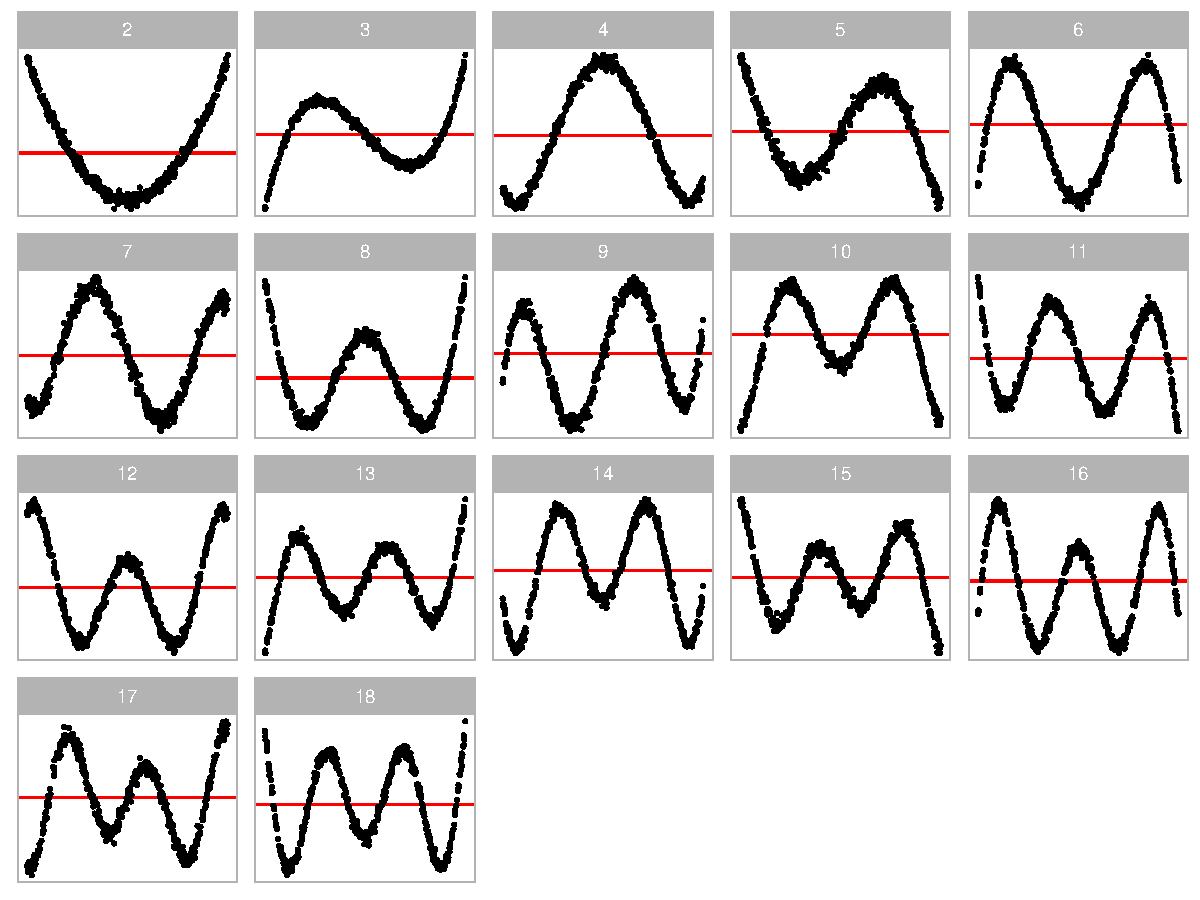
\includegraphics[width=1\linewidth]{appendix_files/figure-latex/different-j-1} 

}

\caption{Non-linearity forms generated for the synthetic data simulation. The 17 shapes are generated by varying the order of polynomial given by $j$ in $He_j(.)$.}\label{fig:different-j}
\end{figure}

Additionally, scaling factor \(\boldsymbol{k}\) directly affects the
error distribution and it is correlated with \(\boldsymbol{x}_1\) and
\(\boldsymbol{x}_2\). If \(b \neq 0\) and
\(\boldsymbol{\varepsilon} \sim N(\boldsymbol{0}_n, \sigma^2\boldsymbol{I}_n)\),
the constant variance assumption will be violated. Parameter \(a\) is a
shape parameter controlling the location of the smallest variance in a
residual plot as shown in Figure \ref{fig:different-a}.

\begin{figure}[!h]

{\centering 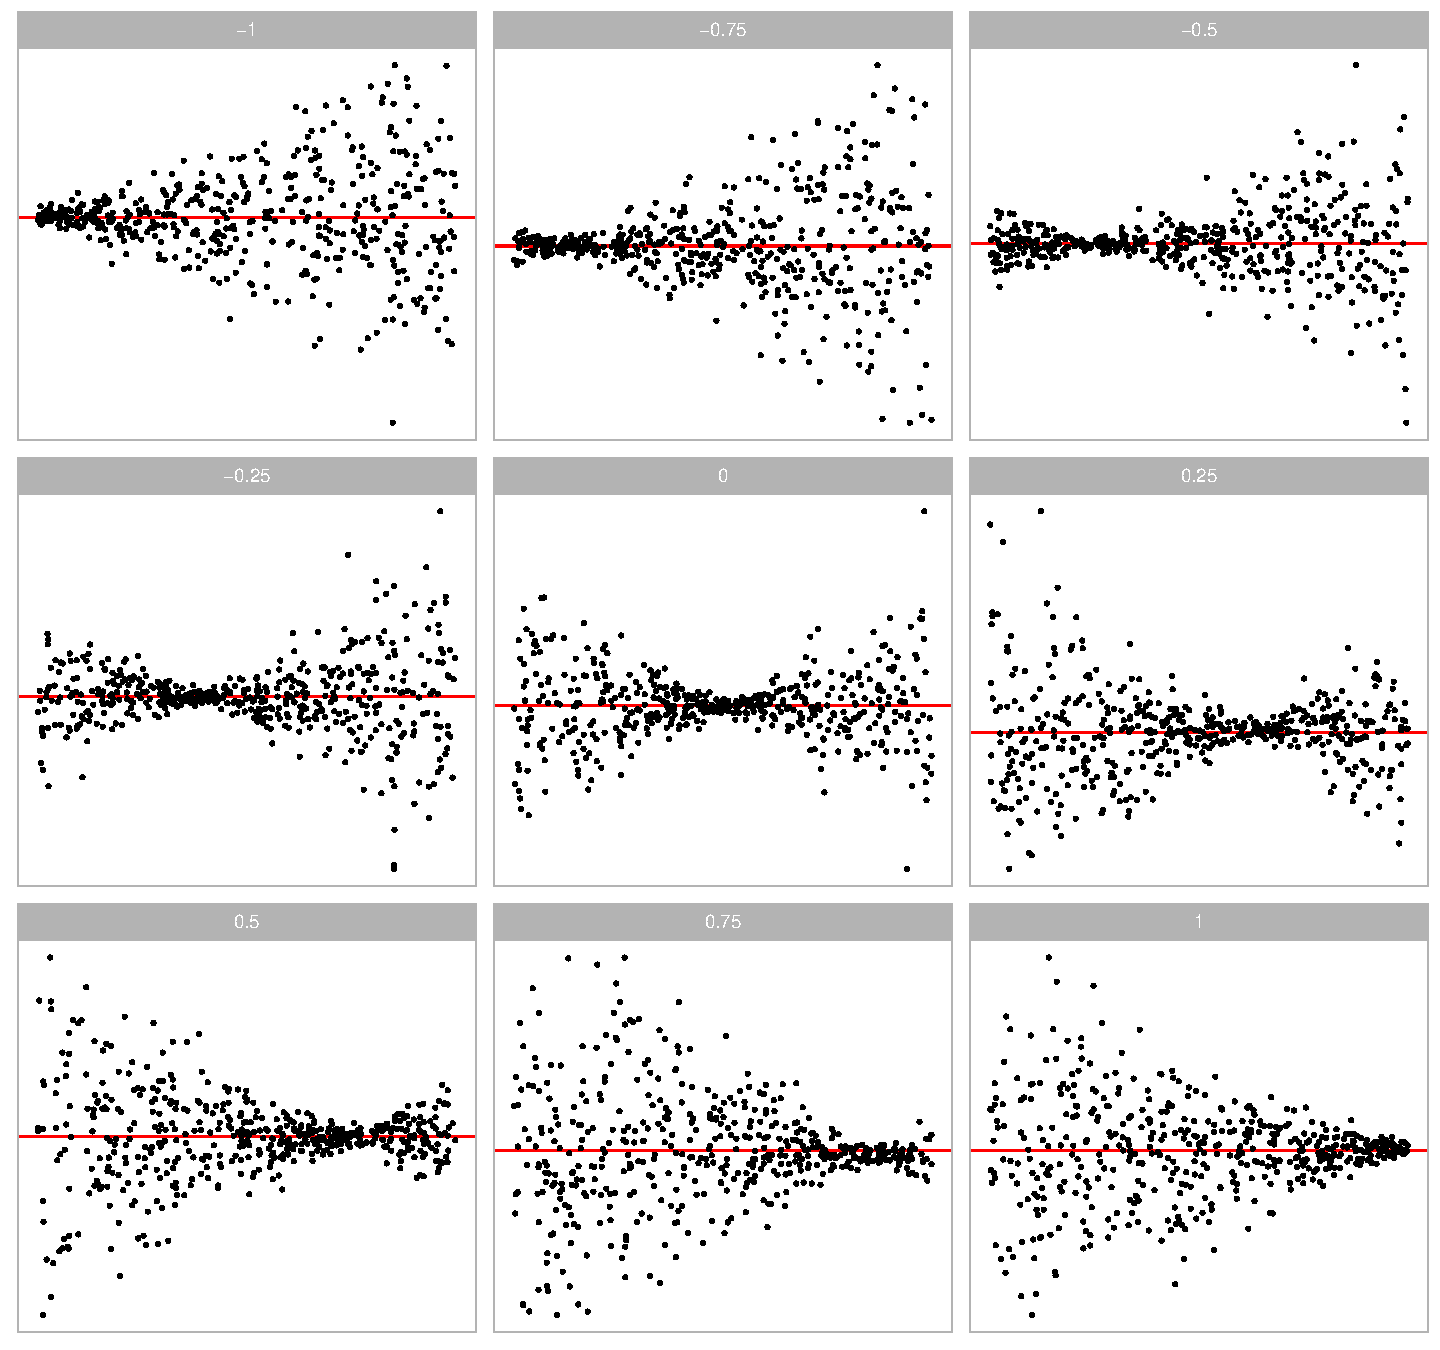
\includegraphics[width=1\linewidth]{appendix_files/figure-latex/different-a-1} 

}

\caption{Heteroskedasticity forms generated for the synthetic data simulation. Different shapes are controlled by the continuous factor $a$ between -1 and 1. For $a = -1$, the residual plot exhibits a "left-triangle" shape. And for $a = 1$, the residual plot exhibits a "right-triangle" shape. }\label{fig:different-a}
\end{figure}

\begin{figure}[!h]

{\centering 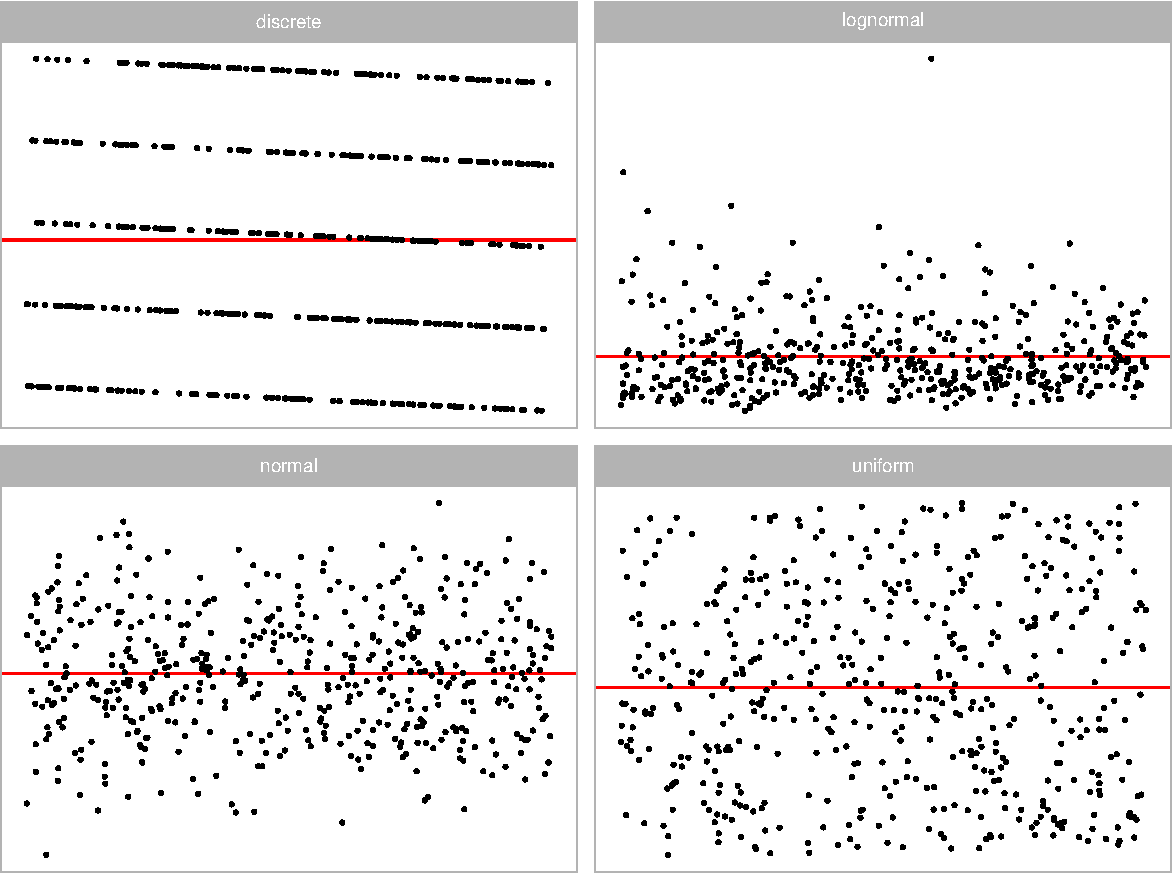
\includegraphics[width=1\linewidth]{appendix_files/figure-latex/different-e-1} 

}

\caption{Non-normality forms generated for the synthetic data simulation. Four different error distributions including discrete, lognormal, normal and uniform are considered.}\label{fig:different-e}
\end{figure}

Non-normality violations arise from specifying a non-normal distribution
for \(\boldsymbol{\varepsilon}\). In the synthetic data simulation, four
distinct error distributions are considered, including discrete,
uniform, normal, and lognormal distributions, as presented in Figure
\ref{fig:different-e}. Each distribution imparts unique characteristics
in the residual plot. The discrete error distribution introduces
discrete clusters in residuals, while the lognormal distribution
typically yields outliers. Uniform error distribution may result in
residuals filling the entire space of the residual plot. All of these
distributions exhibit visual distinctions from the normal error
distribution.

\begin{figure}[!h]

{\centering 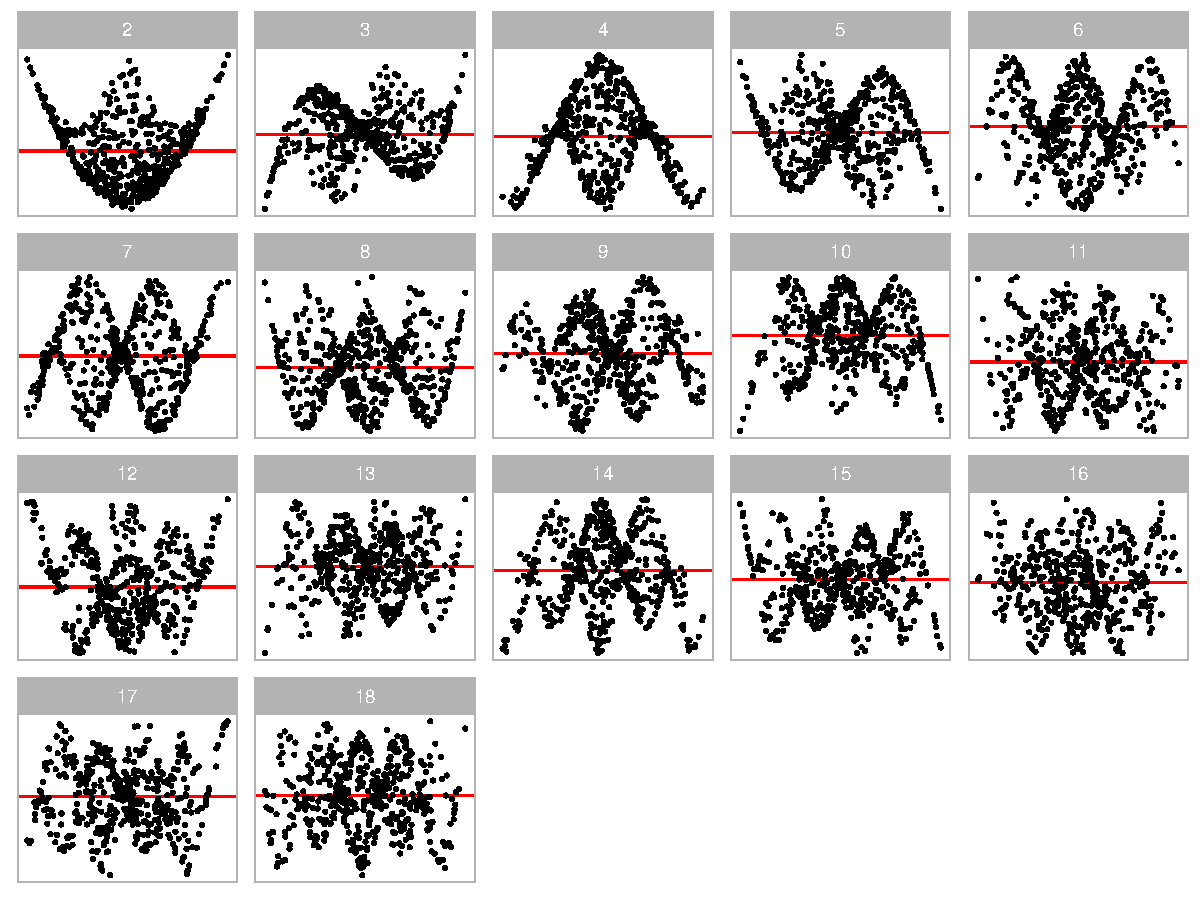
\includegraphics[width=1\linewidth]{appendix_files/figure-latex/different-j-x2-1} 

}

\caption{Residual plots of multiple linear regression models with non-linearity issues. The 17 shapes are generated by varying the order of polynomial given by $j$ in $He_j(.)$. A second predictor $\boldsymbol{x}_2$ is introduced to the regression model to create complex shapes.}\label{fig:different-j-x2}
\end{figure}

\begin{figure}[!h]

{\centering 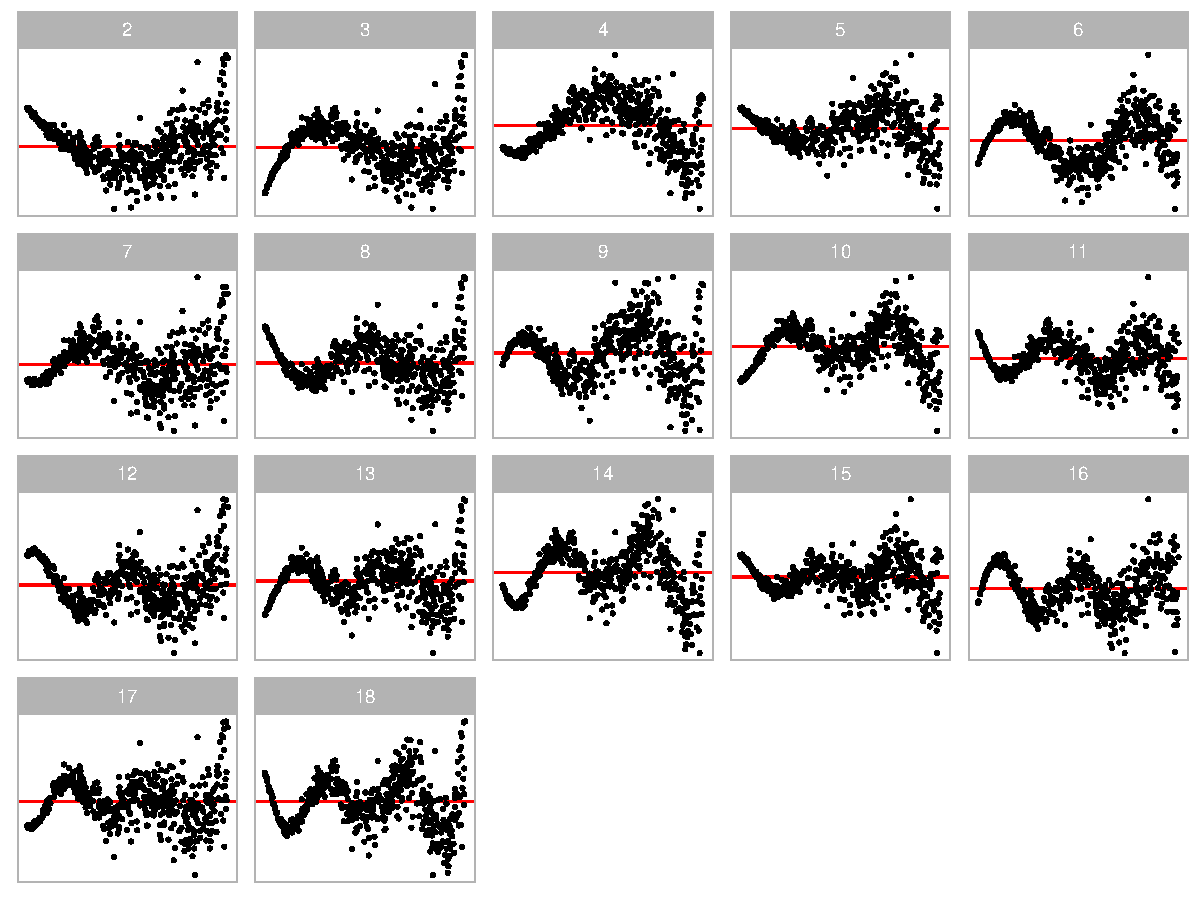
\includegraphics[width=1\linewidth]{appendix_files/figure-latex/different-j-heter-1} 

}

\caption{Residual plots of models violating both the non-linearity and the heteroskedasticity assumptions. The 17 shapes are generated by varying the order of polynomial given by $j$ in $He_j(.)$, and the "left-triangle" shape is introduced by setting $a = -1$.}\label{fig:different-j-heter}
\end{figure}

\begin{figure}[!h]

{\centering 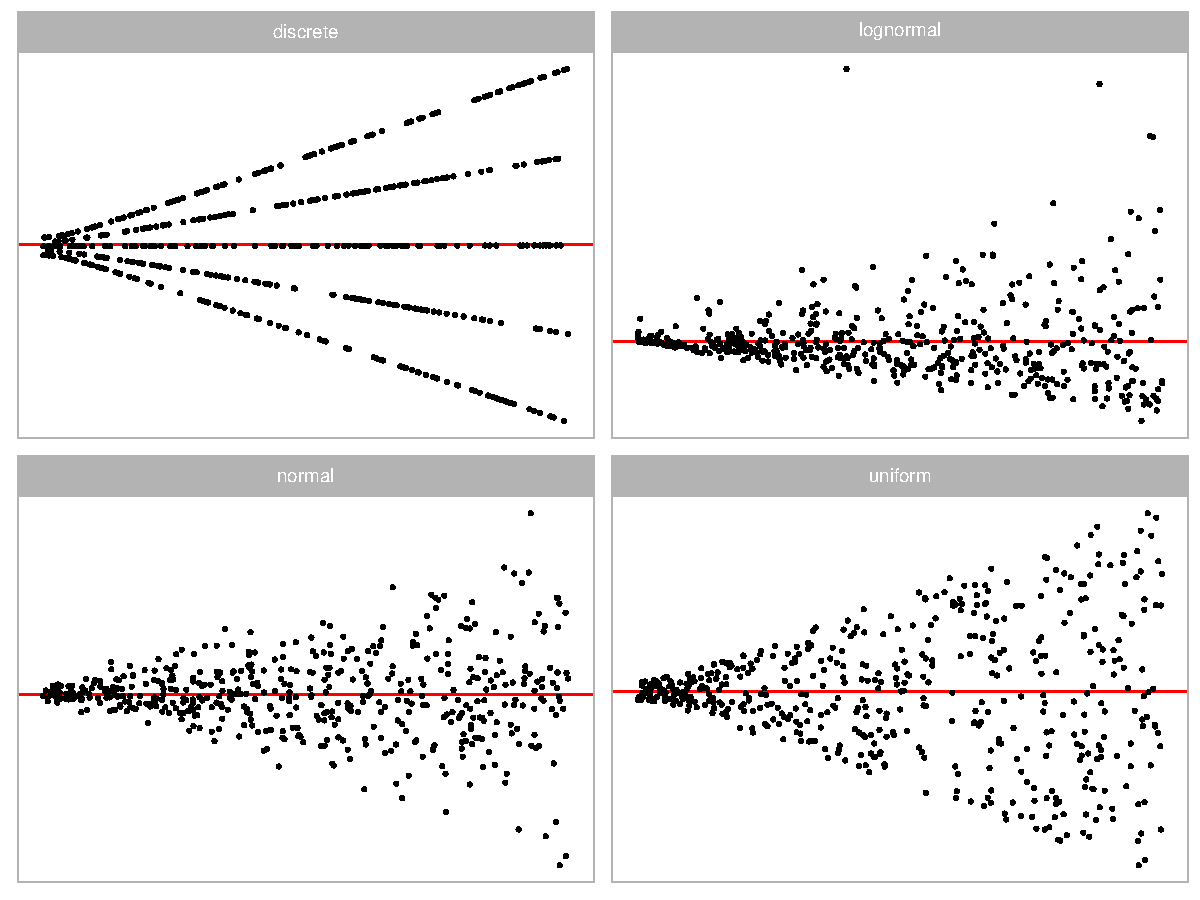
\includegraphics[width=1\linewidth]{appendix_files/figure-latex/different-e-heter-1} 

}

\caption{Residual plots of models violating both the non-normality and the heteroskedasticity assumptions. The four shapes are generated by using four different error distributions including discrete, lognormal, normal and uniform, and the "left-triangle" shape is introduced by setting $a = -1$. }\label{fig:different-e-heter}
\end{figure}

Equation \ref{eq:data-sim} accommodates the incorporation of the second
predictor \(\boldsymbol{x}_2\). Introducing it into the data generation
process by setting \(\beta_1 = 1\) significantly enhances the complexity
of the shapes, as illustrated in Figure \ref{fig:different-j-x2}. In
comparison to Figure \ref{fig:different-j}, Figure
\ref{fig:different-j-x2} demonstrates that the non-linear shape
resembles a surface rather than a single curve. This augmentation can
facilitate the computer vision model in learning visual patterns from
residual plots of the multiple linear regression model.

In real-world analysis, it is not uncommon to encounter instances where
multiple model violations coexist. In such cases, the residual plots
often exhibit a mixed pattern of visual anomalies corresponding to
different types of model violations. Figure \ref{fig:different-j-heter}
and Figure \ref{fig:different-e-heter} show the visual patterns of
models with multiple model violations.

The predictors, \(\boldsymbol{x}_1\) and \(\boldsymbol{x}_2\), are
randomly generated from four distinct distributions, including
\(U(-1, 1)\) (uniform), \(N(0, 0.3^2)\) (normal),
\(\text{lognormal}(0, 0.6^2)/3\) (skewed) and \(U\{-1, 1\}\) (discrete
uniform).

\subsection{Balanced Dataset}\label{balanced-dataset}

To train a robust computer vision model, we deliberately controlled the
distribution of the target variable \(D\) in the training data. We
ensured that it followed a uniform distribution between \(0\) and \(7\).
This was achieved by organizing \(50\) buckets, each exclusively
accepting training samples with \(D\) falling within the range
\([7(i - 1)/49, 7i/49)\) for \(i < 50\), where \(i\) represents the
index of the \(i\)-th bucket. For the \(50\)-th bucket, any training
samples with \(D \geq 7\) were accepted.

With 80,000 training images prepared, each bucket accommodated a maximum
of \(80000/ 50 = 1600\) training samples. The simulator iteratively
sampled parameter values from the parameter space, generated residuals
and fitted values using the data generation process, computed the
distance, and checked if the sample fitted within the corresponding
bucket. This process continued until all buckets were filled.

Similarly, we adopted the same methodology to prepare 8,000 test images
for performance evaluation and model diagnostics.

\bibliographystyle{tfcad}
\bibliography{bibliography.bib}





\end{document}
